% !TEX root = ../main.tex
%!TeX spellcheck = es-CL
\documentclass[../main.tex]{subfiles}

\chapter{Modelos gráficos probabilísticos}

\begin{quotation}
    El \textit{machine learning} fue un objeto de lujo, pero para nosotros es
    un artículo de primera necesidad: no podemos vivir sin \textit{machine learning}.
	\NC{Poner algo profundo por el estilo. (?)}
\end{quotation}

\section*{Introducción}

El eje central de este capitulo se basa en la búsqueda de una representación compacta, para
distribuciones de probabilidad conjunta de la forma $p(\bm x | \bm\theta)$. Esto, con
la intención de realizar inferencia sobre variables y aprendizaje de parámetros de manera
eficiente. \NC{Mejorar intro, añadir discusión sobre inferencia y aprendizaje.}


\section{Modelos gráficos dirigidos}
Toda distribución de probabilidad conjunta $p(\bm x ) = p(x_1, x_2, \ldots x_v)$  se puede
representar de la forma:
\begin{equation}
	\label{eq:regla_cadena}
	p(\bm x ) = p(x_1)p(x_2 \ \vline \ x_1 )p(x_3 \ \vline\  x_1, x_2) \ldots p(x_v\ \vline\  x_1, x_2, \ldots , x_{v-1})
\end{equation}

\NC{discusión sobre computabilidad. (?) (ref: Murphy, pg. 307)}
El problema con esta expresión es la dificultad computacional subyacente al cálculo de
distribuciones condicionales de la forma $p(x_{t} |  x_1,\ldots, x_{t-1} )$
cuando el número de variables incidentes $t$ aumenta.

\NC{propiedades básicas del calculo de probabilidades (CI por ej.) al apéndice.}
No obstante, la representación (\ref{eq:regla_cadena}) reduce su complejidad en presencia de
\index{independencia condicional} \textbf{independencia condicional}.

En efecto, si se asume $x_{t+1} \perp  x_{1}, \ldots, x_{t-1} \ \vline \ x_t$. Es decir,
las observaciones futuras $x_{t+1}$ son independientes del pasado $ x_{1}, \ldots,
x_{t-1}$, dado el estado presente $x_{t}$. La probabilidad conjunta se reduce entonces a:
\begin{equation}
\label{eq:markov_prop}
p(\bm x ) = p(x_1) \prod_{t = 2}^{v} p(x_t  |  x_1,\ldots , x_{t-1}) = p(x_1) \prod_{t = 2}^{v} p(x_t  | x_{t-1})
\end{equation}

De lo cual se obtiene una expresión más simple.

Modelar la independencia condicional entre las variables permite entonces reducir la
complejidad de representación para la distribución conjunta. En particular, la elección tomada
en (\ref{eq:markov_prop}) se conoce como \index{Propiedad de Markov} \textbf{propiedad de
Markov} de primer orden.
En un contexto general, las relaciones de independencia condicional entre variables aleatorias
de dimensión arbitraria, se modelan utilizando \index{Diagramas de
independencia}\textit{diagramas de independencia} o \index{Modelos gráficos}\textbf{modelos
gráficos}. Estos se valen de un grafo $G=(\mathcal{V}, \mathcal{E})$ \footnote{Conjunto
consistente de $\mathcal{V} = \lbrace{1 \ldots , V} \rbrace$ vértices (o nodos) y $\mathcal{E} =
\lbrace {(s,t): s,t \in \mathcal{V}} \rbrace$ aristas.} para
representar mediante nodos $v = 1, \ldots, \mathcal{V}$ las variables aleatorias del modelo,
mientras que la presencia o ausencia de aristas entre estos nodos, permite modelar las
relaciones de dependencia condicional subyacentes.
% Naive Bayes Classifier
\begin{figure}[ht]
\centering
\subfloat[]{\label{fig:grafo_ejemplo}\documentclass[../capitulos/cap1.tex]{subfiles}

\tikzset{every picture/.style={line width=0.75pt}} %set default line width to 0.75pt

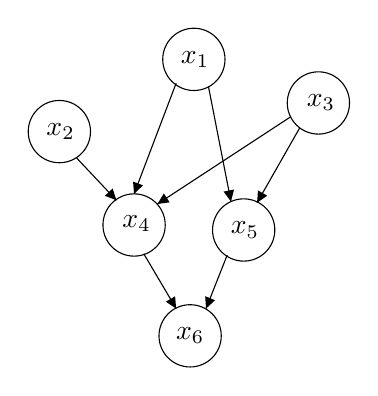
\begin{tikzpicture}[x=0.75pt,y=0.75pt,yscale= -0.6,xscale= 0.6]
%uncomment if require: \path (0,300); %set diagram left start at 0, and has height of 300

\draw    (332, 42) circle [x radius= 25, y radius= 25]  ;
\draw    (224, 100) circle [x radius= 25, y radius= 25]  ;
\draw    (432, 77) circle [x radius= 25, y radius= 25]  ;
\draw    (284, 175) circle [x radius= 25, y radius= 25]  ;
\draw    (372, 179) circle [x radius= 25, y radius= 25]  ;
\draw    (329, 264) circle [x radius= 25, y radius= 25]  ;
\draw    (343.78,64.11) -- (361.78,156.11) ;
\draw [shift={(361.78,156.11)}, rotate = 258.93] [fill={rgb, 255:red, 0; green, 0; blue, 0 }  ] [draw opacity=0] (8.93,-4.29) -- (0,0) -- (8.93,4.29) -- (8.93,-4.29)    ;

\draw    (317.78,61.11) -- (284,150) ;
\draw [shift={(284,150)}, rotate = 290.81] [fill={rgb, 255:red, 0; green, 0; blue, 0 }  ] [draw opacity=0] (8.93,-4.29) -- (0,0) -- (8.93,4.29) -- (8.93,-4.29)    ;

\draw    (237.78,121.11) -- (269.78,155.11) ;
\draw [shift={(269.78,155.11)}, rotate = 226.74] [fill={rgb, 255:red, 0; green, 0; blue, 0 }  ] [draw opacity=0] (8.93,-4.29) -- (0,0) -- (8.93,4.29) -- (8.93,-4.29)    ;

\draw    (417,97) -- (382.78,157.11) ;
\draw [shift={(382.78,157.11)}, rotate = 299.65] [fill={rgb, 255:red, 0; green, 0; blue, 0 }  ] [draw opacity=0] (8.93,-4.29) -- (0,0) -- (8.93,4.29) -- (8.93,-4.29)    ;

\draw    (409.78,88.11) -- (302.78,158.11) ;
\draw [shift={(302.78,158.11)}, rotate = 326.81] [fill={rgb, 255:red, 0; green, 0; blue, 0 }  ] [draw opacity=0] (8.93,-4.29) -- (0,0) -- (8.93,4.29) -- (8.93,-4.29)    ;

\draw    (291.78,198.11) -- (317.78,242.11) ;
\draw [shift={(317.78,242.11)}, rotate = 239.42000000000002] [fill={rgb, 255:red, 0; green, 0; blue, 0 }  ] [draw opacity=0] (8.93,-4.29) -- (0,0) -- (8.93,4.29) -- (8.93,-4.29)    ;

\draw    (358.78,199.11) -- (341.78,242.11) ;
\draw [shift={(341.78,242.11)}, rotate = 291.57] [fill={rgb, 255:red, 0; green, 0; blue, 0 }  ] [draw opacity=0] (8.93,-4.29) -- (0,0) -- (8.93,4.29) -- (8.93,-4.29)    ;


\draw (333,42) node   {$x_{1}$};
\draw (225,100) node   {$x_{2}$};
\draw (434,77) node   {$x_{3}$};
\draw (286,174) node   {$x_{4}$};
\draw (373,179) node   {$x_{5}$};
\draw (329,264) node   {$x_{6}$};


\end{tikzpicture}
}
\quad
\subfloat[]{\label{fig:naive_bayes} \documentclass[../capitulos/cap1.tex]{subfiles}

\tikzset{every picture/.style={line width=0.75pt}} %set default line width to 0.75pt

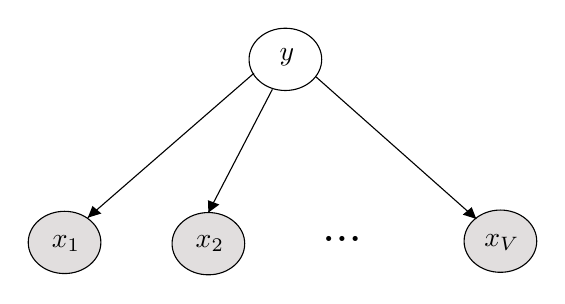
\begin{tikzpicture}[x=0.75pt,y=0.75pt,yscale=-0.6,xscale= 0.7]
%uncomment if require: \path (0,300); %set diagram left start at 0, and has height of 300

\draw    (338, 37) circle [x radius= 25, y radius= 25]  ;
\draw  [fill={rgb, 255:red, 225; green, 222; blue, 222 }  ,fill opacity=1 ]  (285, 185) circle [x radius= 25, y radius= 25]  ;
\draw  [fill={rgb, 255:red, 225; green, 222; blue, 222 }  ,fill opacity=1 ]  (186, 184) circle [x radius= 25, y radius= 25]  ;
\draw  [fill={rgb, 255:red, 225; green, 222; blue, 222 }  ,fill opacity=1 ]  (486, 183) circle [x radius= 25, y radius= 25]  ;
\draw    (316.38,48.11) -- (202.02,164.11) ;
\draw [shift={(202.02,164.11)}, rotate = 314.59000000000003] [fill={rgb, 255:red, 0; green, 0; blue, 0 }  ] [draw opacity=0] (8.93,-4.29) -- (0,0) -- (8.93,4.29) -- (8.93,-4.29)    ;

\draw    (329.02,61.11) -- (285,160) ;
\draw [shift={(285,160)}, rotate = 293.99] [fill={rgb, 255:red, 0; green, 0; blue, 0 }  ] [draw opacity=0] (8.93,-4.29) -- (0,0) -- (8.93,4.29) -- (8.93,-4.29)    ;

\draw    (359,51) -- (469.38,165.11) ;
\draw [shift={(469.38,165.11)}, rotate = 225.95] [fill={rgb, 255:red, 0; green, 0; blue, 0 }  ] [draw opacity=0] (8.93,-4.29) -- (0,0) -- (8.93,4.29) -- (8.93,-4.29)    ;


\draw (377,181) node [scale=1.7280000000000002] [align=left] {...};
\draw (339,35) node   {$y$};
\draw (187,185) node   {$x_{1}$};
\draw (286,185) node   {$x_{2}$};
\draw (487,184) node   {$x_{V}$};


\end{tikzpicture}
}
\caption{\subref{fig:grafo_ejemplo} Ejemplo de modelo gráfico dirigido.
\subref{fig:naive_bayes} Relaciones de dependencia condicional en el clasificador
 naive Bayes como un modelo gráfico dirigido, las variables aleatorias observadas
 se denotan por nodos grises.}
\end{figure}

Una \index{Red bayesiana} \textit{red bayesiana} o \index{modelo gráfico dirigido}\textbf{modelo
gráfico dirigido} es un modelo gráfico probabilístico, cuyo grafo subyacente es un \index{grafo
dirigido acíclico} \textbf{grafo dirigido acíclico} (\index{DAG}DAG por sus siglas en ingles).
Todo DAG posee un \index{ordenamiento topológico} \textit{ordenamiento topológico}, es decir,
los nodos de cualquier DAG pueden ser numerados de manera tal, que todo nodo padre
posea una numeración inferior a sus nodos hijos. \NC{lema de ordenamiento topológico
para DAG's en apéndice.} Esta característica permite enriquecer la formulación de la propiedad
de Markov (\ref{eq:markov_prop}), usando la estructura grafica como componente adicional. De
esta forma, se puede formular la \index{propiedad ordenada de Markov} \textbf{propiedad ordenada
de Markov} en modelos gráficos dirigidos:
\begin{equation}
	\label{eq:Markov_ordenado}
	x_s \perp \bm x_{pred(s) \setminus pa(s)} ~ | ~ \bm x_{pa(s)}
\end{equation}

Es decir, un nodo $x_s$ es independiente de aquellos predecesores, menores en orden topológico,
a sus padres $ \bm x_{pred(s) \setminus pa(s)}$, dados sus nodos padres $\bm x_{pa(s)}$. De
manera equivalente, un nodo $x_s$ solo depende de sus padres inmediatos $x_{pa(s)}$ y no de
todos sus predecesores.

De esta forma, la probabilidad conjunta de un modelo gráfico dirigido, que cumple la propiedad
ordenada de Markov, se puede descomponer de la forma:
\begin{equation}
\label{eq:markov_prop_ord}
p(\bm x ) = \prod_{t = 1}^{V} p(x_t  |  \bm x_{pa(t)})
\end{equation}

\begin{example}[Modelo grafico asociado a $p(\bm x)$]
Si se estudia un modelo probabilístico, donde la probabilidad conjunta de las variables
estudiadas $p(\bm x)$ esta dada por:
\begin{equation}
\label{eq:conj_grafo_ejemplo}
p(\bm x) = p(x_1)p(x_2)p(x_3)p(x_4 | x_1, x_2, x_3)p(x_5 | x_1, x_3)p(x_6 | x_4, x_5)
\end{equation}

Entonces, un grafo dirigido asociado a tal factorización es el de la figura
\ref{fig:grafo_ejemplo}. Para construir dicho grafo, se consideran las relaciones de
independencia condicional en la factorización (\ref{eq:conj_grafo_ejemplo}), para luego
establecer aristas $s \rightarrow t$ si la probabilidad condicional del nodo $x_s$ depende de
$x_t$. En este caso, no hay aristas incidentes hacia $x_1$, $x_2$ ni $x_3$. Por otra parte, se
deben crear aristas desde $x_1, x_2$ y $x_3$ hacia $x_4$, desde $x_1$ y $x_3$ hacia $x_5$ y
desde $x_4, x_5$ hacia $x_6$.

En general, es posible reconstruir la probabilidad conjunta subyacente a un modelo
gráfico probabilístico conociendo el grafo y haciendo el proceso inverso al descrito
anteriormente.
\end{example}

Con el fin de explorar las posibilidades de este tipo de modelos e introducir conceptos
 referentes a la notación de estos, se pasan a estudiar los siguientes ejemplos:

\subsection{Naive Bayes}
\index{Naive Bayes}

Dado un problema de clasificación de vectores $\bm x = (x_1, \ldots , x_V)$ en $C$ clases. Es
posible modelar las variables de decisión $x_t$ como condicionalmente independientes dada la
categoría de clasificación:
\begin{equation}
	\label{eq:cond_nb}
	x_i \perp x_j ~| y =  c, ~~ i \neq j
\end{equation}

Si se usa este enfoque, se obtiene que la densidad condicional de clases toma la forma:
\begin{equation}
	\label{eq:naive_bayes}
	p(\bm x ~ | y = c) = \prod_{t=1}^{V}p(x_t ~ | y = c)
\end{equation}

Al parametrizar las distribuciones de densidad condicional, es posible obtener un modelo de
clasificación conocido como \index{clasificador naive Bayes}\textbf{clasificador naive Bayes}.
 La estructura de las relaciones de independencia inducidas por (\ref{eq:cond_nb}) se pueden
expresar según (\ref{eq:naive_bayes}) y el modelo gráfico dirigido de la figura \ref{fig:naive_bayes}.

\subsection{Regresión polinomial}
\NC{añadir intro significativa}
las variables aleatorias son el vector de coeficientes polinomiales $\bm w$ y los
datos observados $\bm y = (y_1 , \ldots , y_N)^{T}$. Adicionalmente, se parametriza
el ruido del modelo a través de $\sigma_{\varepsilon}^2$ y la varianza de la distribución
a priori \footnote{Considerándose una distribución a priori, gaussiana y esférica sobre $\bm w$.}
de $\bm w$ por $\sigma_w^2$. Finalmente, los datos de entrada se denotan por
$\bm x = (x_1 , \ldots , x_N)^{T}$.

La probabilidad conjunta de este modelo es el producto de la probabilidad
a priori $p(\bm w)$ con las distribuciones condicionales $p(y_i  |  \bm w)$
para $i = 1, \ldots, N$:
\begin{equation}
    \label{eq:poly_fact_1}
 p(\bm y, \bm w ) = p(\bm w) \prod_{i = 1}^{N} p(y_i  | \bm w)
\end{equation}

El grafo de tal factorización es similar al del clasificador naive Bayes \ref{fig:naive_bayes}.
Para representarlo de manera compacta, se usa la notación de de placas o \textit{plates},
en la figura \ref{fig:plate_poly_graph} se muestra el grafo de (\ref{eq:poly_fact_1})
usando esta convención. Aquí $N$ es la cantidad de nodos del modelo, de los cuales se muestra
el representante $y_i$.

\begin{figure}[ht]
\subfloat[]{\label{fig:plate_poly_graph}\documentclass[../capitulos/cap1.tex]{subfiles}

\tikzset{every picture/.style={line width=0.75pt}} %set default line width to 0.75pt

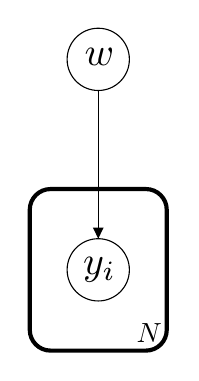
\begin{tikzpicture}[x=0.75pt,y=0.75pt,yscale=-0.6,xscale=0.6]
%uncomment if require: \path (0,300); %set diagram left start at 0, and has height of 300

\draw    (316, 50) circle [x radius= 25, y radius= 25]  ;
\draw    (316, 219) circle [x radius= 25, y radius= 25]  ;
\draw    (316,75) -- (316,194) ;
\draw [shift={(316,194)}, rotate = 270] [fill={rgb, 255:red, 0; green, 0; blue, 0 }  ] [draw opacity=0] (8.93,-4.29) -- (0,0) -- (8.93,4.29) -- (8.93,-4.29)    ;

\draw  [line width=1.5]  [rounded corners= 7.5] (261, 154.14) rectangle (371, 283.86)   ;

\draw (317,48) node [scale=1.44]  {$\boldsymbol{w}$};
\draw (317,219) node [scale=1.44]  {$y_{i}$};
\draw (357,270) node   {$N$};


\end{tikzpicture}
}
\quad
\subfloat[]{\label{fig:plate_poly_graph_2}\tikzset{every picture/.style={line width=0.75pt}} %set default line width to 0.75pt        

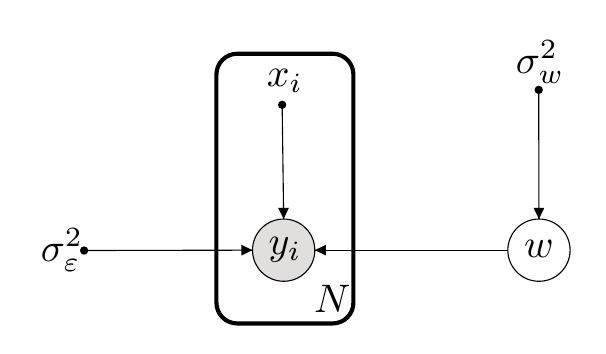
\begin{tikzpicture}[x=0.75pt,y=0.75pt,yscale=-0.6,xscale=0.6]
%uncomment if require: \path (0,300); %set diagram left start at 0, and has height of 300

\draw    (521, 219) circle [x radius= 25, y radius= 25]  ;
\draw  [fill={rgb, 255:red, 225; green, 222; blue, 222 }  ,fill opacity=1 ]  (316, 219) circle [x radius= 25, y radius= 25]  ;
\draw    (496,219) -- (341,219) ;
\draw [shift={(341,219)}, rotate = 360] [fill={rgb, 255:red, 0; green, 0; blue, 0 }  ] [draw opacity=0] (8.93,-4.29) -- (0,0) -- (8.93,4.29) -- (8.93,-4.29)    ;

\draw  [line width=1.5]  [rounded corners= 7.5] (262, 61.29) rectangle (372, 277.86)   ;
\draw    (155.78,219.29) -- (291,219) ;
\draw [shift={(291,219)}, rotate = 539.88] [fill={rgb, 255:red, 0; green, 0; blue, 0 }  ] [draw opacity=0] (8.93,-4.29) -- (0,0) -- (8.93,4.29) -- (8.93,-4.29)    ;
\draw [shift={(155.78,219.29)}, rotate = 359.88] [fill={rgb, 255:red, 0; green, 0; blue, 0 }  ] [draw opacity=0]    (0, 0) circle [x radius= 3.35, y radius= 3.35]   ;
\draw    (520.78,90.29) -- (521,194) ;
\draw [shift={(521,194)}, rotate = 269.88] [fill={rgb, 255:red, 0; green, 0; blue, 0 }  ] [draw opacity=0] (8.93,-4.29) -- (0,0) -- (8.93,4.29) -- (8.93,-4.29)    ;
\draw [shift={(520.78,90.29)}, rotate = 89.88] [fill={rgb, 255:red, 0; green, 0; blue, 0 }  ] [draw opacity=0]    (0, 0) circle [x radius= 3.35, y radius= 3.35]   ;
\draw    (314.78,102.29) -- (316,194) ;
\draw [shift={(316,194)}, rotate = 269.24] [fill={rgb, 255:red, 0; green, 0; blue, 0 }  ] [draw opacity=0] (8.93,-4.29) -- (0,0) -- (8.93,4.29) -- (8.93,-4.29)    ;
\draw [shift={(314.78,102.29)}, rotate = 89.24] [fill={rgb, 255:red, 0; green, 0; blue, 0 }  ] [draw opacity=0]    (0, 0) circle [x radius= 3.35, y radius= 3.35]   ;

\draw (521,218) node [scale=1.44]  {$\boldsymbol{w}$};
\draw (317,219) node [scale=1.44]  {$y_{i}$};
\draw (355,258) node [scale=1.44]  {$N$};
\draw (138,219) node [scale=1.44]  {$\sigma ^{2}_{\varepsilon }$};
\draw (522,68) node [scale=1.44]  {$\sigma ^{2}_{w}$};
\draw (317,83) node [scale=1.44]  {$x_{i}$};


\end{tikzpicture}
}
\quad
\subfloat[]{\label{fig:plate_poly_graph_final}\tikzset{every picture/.style={line width=0.75pt}} %set default line width to 0.75pt

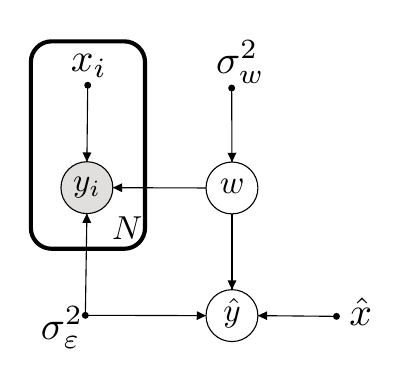
\begin{tikzpicture}[x=0.75pt,y=0.75pt,yscale=-0.5,xscale=0.5]
%uncomment if require: \path (0,350); %set diagram left start at 0, and has height of 350

\draw    (208.5,285) -- (210,187) ;
\draw [shift={(210,187)}, rotate = 450.88] [fill={rgb, 255:red, 0; green, 0; blue, 0 }  ] [draw opacity=0] (8.93,-4.29) -- (0,0) -- (8.93,4.29) -- (8.93,-4.29)    ;
\draw [shift={(208.5,285)}, rotate = 270.88] [fill={rgb, 255:red, 0; green, 0; blue, 0 }  ] [draw opacity=0]    (0, 0) circle [x radius= 3.35, y radius= 3.35]   ;
\draw    (349.78, 162.29) circle [x radius= 25, y radius= 25]  ;
\draw  [fill={rgb, 255:red, 225; green, 222; blue, 222 }  ,fill opacity=1 ]  (210, 162) circle [x radius= 25, y radius= 25]  ;
\draw    (324.78,162.29) -- (235,162) ;
\draw [shift={(235,162)}, rotate = 360.18] [fill={rgb, 255:red, 0; green, 0; blue, 0 }  ] [draw opacity=0] (8.93,-4.29) -- (0,0) -- (8.93,4.29) -- (8.93,-4.29)    ;

\draw  [line width=1.5]  [rounded corners= 7.5] (156, 21) rectangle (266, 220.86)   ;
\draw    (349.5,66) -- (349.78,137.29) ;
\draw [shift={(349.78,137.29)}, rotate = 269.77] [fill={rgb, 255:red, 0; green, 0; blue, 0 }  ] [draw opacity=0] (8.93,-4.29) -- (0,0) -- (8.93,4.29) -- (8.93,-4.29)    ;
\draw [shift={(349.5,66)}, rotate = 89.77] [fill={rgb, 255:red, 0; green, 0; blue, 0 }  ] [draw opacity=0]    (0, 0) circle [x radius= 3.35, y radius= 3.35]   ;
\draw    (210.78,63.29) -- (210,137) ;
\draw [shift={(210,137)}, rotate = 270.61] [fill={rgb, 255:red, 0; green, 0; blue, 0 }  ] [draw opacity=0] (8.93,-4.29) -- (0,0) -- (8.93,4.29) -- (8.93,-4.29)    ;
\draw [shift={(210.78,63.29)}, rotate = 90.61] [fill={rgb, 255:red, 0; green, 0; blue, 0 }  ] [draw opacity=0]    (0, 0) circle [x radius= 3.35, y radius= 3.35]   ;
\draw    (349.78, 285.29) circle [x radius= 25, y radius= 25]  ;
\draw    (208.5,285) -- (324.78,285.29) ;
\draw [shift={(324.78,285.29)}, rotate = 180.14] [fill={rgb, 255:red, 0; green, 0; blue, 0 }  ] [draw opacity=0] (8.93,-4.29) -- (0,0) -- (8.93,4.29) -- (8.93,-4.29)    ;

\draw    (349.78,187.29) -- (349.78,260.29) ;
\draw [shift={(349.78,260.29)}, rotate = 270] [fill={rgb, 255:red, 0; green, 0; blue, 0 }  ] [draw opacity=0] (8.93,-4.29) -- (0,0) -- (8.93,4.29) -- (8.93,-4.29)    ;

\draw    (450.5,286) -- (374.78,285.29) ;
\draw [shift={(374.78,285.29)}, rotate = 360.53999999999996] [fill={rgb, 255:red, 0; green, 0; blue, 0 }  ] [draw opacity=0] (8.93,-4.29) -- (0,0) -- (8.93,4.29) -- (8.93,-4.29)    ;
\draw [shift={(450.5,286)}, rotate = 180.54] [fill={rgb, 255:red, 0; green, 0; blue, 0 }  ] [draw opacity=0]    (0, 0) circle [x radius= 3.35, y radius= 3.35]   ;

\draw (210,162) node [scale=1.2]  {$y_{i}$};
\draw (249,201) node [scale=1.2]  {$N$};
\draw (186,297) node [scale=1.44]  {$\sigma ^{2}_{\varepsilon }$};
\draw (358,41) node [scale=1.44]  {$\sigma ^{2}_{w}$};
\draw (212,45) node [scale=1.44]  {$x_{i}$};
\draw (474,281) node [scale=1.44]  {$\hat{x}$};
\draw (350,283) node [scale=1.2]  {$\hat{y}$};
\draw (350,161) node [scale=1.2]  {$\boldsymbol{w}$};


\end{tikzpicture}
}
\caption{ Modelo grafico dirigido para regresión
polinomial usando notación de placas (o \textit{plates}). En \subref{fig:plate_poly_graph}
se muestra el grafo correspondiente a (\ref{eq:poly_fact_1}). En \subref{fig:plate_poly_graph_2}
se añaden los parámetros deterministas y las variables aleatorias observadas. En
\subref{fig:plate_poly_graph_final} se añaden datos de entrada y predicciones.}
\end{figure}

Si por otra parte, si se quiere estudiar la interacción de los parámetros en el modelo,
es posible explicitarlos en la probabilidad conjunta para luego agregarlos al grafo:
\begin{equation}
\label{eq:poly_fact_2}
p(\bm y, \bm w | \bm x, \sigma_\varepsilon^2, \sigma_w^2 ) =
p(\bm w | \sigma_w^2) \prod_{i = 1}^{N} p(y_i | \bm w, x_i, \sigma_\varepsilon^2)
\end{equation}

La figura \ref{fig:plate_poly_graph_2} muestra el grafo correspondiente a (\ref{eq:poly_fact_2}).
Por convención, las variables deterministas se incluyen en el grafo como círculos
pequeños, mientras que las variables aleatorias observadas se muestran como nodos grises,
los nodos incoloros representan variables latentes o no observadas, finalmente las
aristas, al igual que en los ejemplos anteriores, representan la dependencia condicional
en la factorización de la probabilidad conjunta.
\NC{ver si es necesario cambiar el formato de los 3 grafos juntos. (muy pegados ?)}

Para realizar predicciones en datos nuevos $\hat{x}$, se desea encontrar la distribución
de probabilidad para $\hat{y}$ condicionada a la información que ya se posee. Esta
corresponde a:
\begin{equation}
    \label{eq:ploy_conj_pred_0}
    p(\hat{y}, \bm y, \bm w | \hat{x}, \bm x, \sigma_w^2, \sigma_\varepsilon^2)
    = \left[ \prod_{i=1}^{N}p(y_i | x_i, \bm w, \sigma_\varepsilon^2) \right]
    p(\bm w | \sigma_w^2) p(\hat{y} | \hat{x}, \bm w, \sigma_\varepsilon^2)
\end{equation}

Finalmente, se deduce la distribución predictiva para $\hat{y}$ :
\begin{equation}
    \label{eq:ploy_pred}
    p(\hat{y}| \hat{x}, \bm y, \bm x, \sigma_w^2, \sigma_\varepsilon^2)
    \propto \int p(\hat{y}, \bm y, \bm w | \hat{x}, \bm x,  \sigma_w^2,
    \sigma_\varepsilon^2) ~ d \bm w
\end{equation}

El modelo gráfico dirigido que encapsula estas últimas ecuaciones se aprecia en
\ref{fig:plate_poly_graph_final}.

\subsection{Modelos gráficos dirigidos gaussianos}

Sea $\mathcal{M}$ un modelo grafico dirigido, en el cual todas las variables son
reales y sus distribuciones de probabilidad condicional son lineal-gaussianas:
\begin{equation}
	\label{eq:gaussian_cpd}
	p(x_t  |  \bm x_{pa(t)}) = \mathcal{N}(x_t  |  \mu_t + \bm w_{t}^T \bm x_{pa(t)}, \sigma_t^2)
\end{equation}

La estructura de $\mathcal{M}$ permite modelar la probabilidad conjunta de las
variables del modelo en la forma:
\begin{equation}
	\label{eq:ver_red_bayesiana_gaussiana}
	p(\bm x  | \mathcal{M}) = \prod_{t=1}^{V} p(x_t  |  \bm x_{pa(t)}) =  \mathcal{N}(\bm x  |  \bm \mu , \Sigma)
\end{equation}

Lo cual se conoce como \index{red bayesiana gaussiana} \textbf{red bayesiana gaussiana}.
Para este tipo de modelos, es posible inferir
$\bm \mu$ y $ \bm \Sigma$. En efecto, según (\ref{eq:ver_red_bayesiana_gaussiana}):
\begin{equation}
	\label{eq:log_gaussian_cpd}
	 \log p( \bm x  |  \mathcal{M}) = - \sum_{t = 1}^{V} \frac{1}{2\sigma_t^2} \left(
	 x_t - \sum_{s \in pa(t)} w_{ts}  x_s - \mu_t	 \right)^2 + K
\end{equation}

Donde $K$ representa una constante independiente de de $\bm x$. Al ser la log-probabilidad
conjunta, cuadrática en las componentes de $\bm x$, se obtiene que efectivamente la
probabilidad conjunta es normal multivariada para  $\bm x$ en
(\ref{eq:ver_red_bayesiana_gaussiana}). Para estimar la media, se observa en primera instancia:
\begin{equation}
	\label{eq:E_x}
	x_t = \sum_{s \in pa(t)} w_{ts} \mathbb{E}[x_s] + \mu_t + \sigma_t \varepsilon_t
\end{equation}

Donde $\varepsilon_t \sim \mathcal{N}(0,1)$ y $\mathbb{E}[\varepsilon_t, \varepsilon_s] =  0 $,
para $s \neq t$. De esto se deduce:
\begin{equation}
\label{eq:E_x_2}
\mathbb{E}[x_t] = \sum_{s \in pa(t)} w_{ts} \mathbb{E}[x_s] + \mu_t
\end{equation}

Es posible entonces, encontrar las componentes de $\bm \mu =\mathbb{E}[\bm x]
=(\mathbb{E}[x_1], \ldots, \mathbb{E}[x_V])^T$ utilizando la estructura gráfica
dirigida de $\mathcal{M}$ (y por tanto su ordenamiento topológico). Para ello, se
comienza calculando $\mathbb{E}[x_1]$ para luego
continuar de manera recursiva según la numeración de los nodos.

Similarmente, es posible calcular el elemento $\bm \Sigma_{st}$ de la matriz de
covarianza, observando:
\begin{align}
    \label{eq:E_cov}
    \text{cov}(x_s,x_t) &= \mathbb{E}[(x_s - \mathbb{E}[x_s])(x_t - \mathbb{E}[x_t])] \nonumber \\
                        &= \left[ (x_s - \mathbb{E}[x_s]) \left\lbrace {\sum_{k \in pa(x_t)} w_{tk} (x_k - \mathbb{E}[x_k]) + \sigma_t \varepsilon_t} \right\rbrace \right]\\
                        &= \sum_{k \in pa(x_t)} w_{tk} ~ \text{cov}[x_s, x_t] + \sigma_t^2 \bm I_{st} \nonumber
\end{align}

De donde al igual que en (\ref{eq:E_x_2}), se calculan los elementos de $\bm \Sigma$
recursivamente.

Finalmente, se puede extender el modelo inducido por (\ref{eq:gaussian_cpd}) a uno
donde los nodos del modelo gráfico representen variables aleatorias gaussianas
multivariantes. Para esto, se reescribe la distribución de probabilidad condicional
para el nodo $x_t$ en la forma:
\begin{equation}
    \label{eq:gaussian_cpd_multi}
	p(\bm x_t ~ | ~ pa(\bm x_t)) =  \mathcal{N}\left( \bm x_t ~  \vline height 4ex
    depth 10pt \sum_{s \in pa(\bm x_t)} \bm W_{ts} \bm x_s + \bm \mu_t~, \bm \Sigma_t \right)
\end{equation}

Donde $\bm W_{ts}$ es una matriz de pesos entre los vectores de cada nodo.

\section{Independencia condicional en modelos gráficos dirigidos}

Como se mencionó anteriormente, los modelos gráficos encapsulan las relaciones
de independencia condicional entre las variables aleatorias del fenómeno que
se modela. En esta sección se estudian las propiedades de los modelos gráficos
dirigidos en cuanto sus propiedades \NC{terminar intro}

En un grafo $G$, se escribe $x_i \perp_{G} x_j | x_k$ si el nodo
$x_i$ es independiente de $x_j$ dado $x_k$. Se denota por $I(G)$ al conjunto
de todas las relaciones de independencia condicional codificadas en el grafo $G$.

\begin{definition}[Diagrama de independencia]
\label{def:diagrama_independencia}
Sea $p(\cdot)$ una distribución de probabilidad. Se dice que un grafo $G$ es un
diagrama de independencia o \textit{I-map}  para $p$ si y solo si $I(G) \subseteq I(p)$.
Donde $I(p)$ es el conjunto de todas las relaciones de independencia condicional
ciertas para las variables de $p$.
\end{definition}

De la definición anterior, se deduce que un grafo $G$ es un diagrama de independencia
para la distribución de probabilidad $p$, si este no contiene más relaciones de
independencia condicional que las permitidas por $p$. De esta forma, toda distribución
de probabilidad $p(\bm x)$, donde $\bm x = (x_1, ..., x_V)^T$, posee al menos un
diagrama de independencia. En efecto, si se considera un grafo $G$ con nodos
$\mathcal{V} = \lbrace{x_1, ..., x_V}\rbrace$ completamente conectados, entonces
$G$ es un diagrama de independencia para $p$ pues no presenta aristas faltantes y
por tanto se condiciona en todas las variables.

De la discusión anterior, tiene sentido hablar de un \textit{diagrama de independencia minimal}
$G$ para $p$, es decir, un grafo $G$, tal que si $G'$ es otro diagrama de independencia
para $p$ que cumple  $G' \subseteq G$, entonces $G' = G$.

Finalmente, tal representación, permite extraer de su estructura gráfica, relaciones
no triviales de independencia condicional, entre las variables de importancia. En el
caso de un modelo gráfico dirigido, la noción de \textit{separación dirigida}
o \textit{d-separación} facilita dicha tarea.

\subsection{d-separación}

Se dice que un \textit{camino no dirigido} $P$ esta \textit{separado de manera dirigida}
o \textit{d-separado} por un conjunto de nodos $E$, si y solo si, se cumple alguna
de las siguiente condiciones:
\begin{enumerate}
    \item $P$ contiene una cadena, $s \rightarrow e \rightarrow t$, donde $e \in E$.
    \item $P$ contiene una estructura $s \leftarrow e \rightarrow t$, donde $e \in E$.
    \item $P$ contiene una estructura $s \rightarrow e \leftarrow t$, donde $e \notin E$
    o $e$ \textbf{no} es descendiente de algún elemento de $E$.
\end{enumerate}

Se dice que un conjunto de nodos $A$ esta d-separado de un conjunto de nodos $B$,
dado un conjunto de nodos $E$, si y solo si, todo camino no dirigido desde cada nodo
de $A$ a cada nodo de $B$ esta d-separado por $E$.

En un grafo acíclico dirigido $G$, se aprecia la siguiente propiedad:
%\begin{flalign}
%    \label{eq:global_markov}
%\bm x_A \perp_G \bm x_B | \bm x_E \iff A \text{ esta d-separado de } $B$ \text{ dado } E
%\end{flalign}

Para comprender las propiedades anteriores, se analizan los siguientes ejemplos:

\begin{itemize}
    \item Sea $x \rightarrow y \rightarrow z$ una cadena, tal grafo codifica la
    siguiente probabilidad conjunta:
    \begin{equation*}
        p(x,y,z) = p(x) p(y | x)p(z | y)
    \end{equation*}
    Usando la propiedad (1), se puede deducir que $x \perp z | y$. Esto se comprueba
    pues:
    \begin{equation*}
    p(x,z | y) = \frac{p(x, y, z)}{p(y)} = \frac{p(x) p(y | x) p(z | y)}{p(y)}
    = \frac{p(x,y) p(z | y)}{p(y)}= p(x|y)p(z|y)
    \end{equation*}

    \item Sea la estructura $x \leftarrow y \rightarrow z$, según la propiedad (2),
    $x \perp z | y$. En efecto,
    \begin{equation*}
    p(x, z | y) = \frac{p(x, y, z)}{p(y)} = \frac{p(y)p(x|y)p(z|y)}{p(y)} =p(x|y)p(z|y)
    \end{equation*}

    \item Sea finalmente la estructura $x \rightarrow y \leftarrow z$, en este caso
    $x \not\perp z | y$ :
    \begin{equation*}
    p(x, z | y) = \frac{p(x, y, z)}{p(y)} = \frac{p(x)p(y|x,z)p(z)}{p(y)} \neq p(x|y)p(z|y)
    \end{equation*}
    Es por tal motivo que en la propiedad (3), se requiere en este tipo de estructuras,
    que no existan nodos, ni descendientes de nodos de la familia condicionante $E$.
\end{itemize}

En el último caso, se puede comprobar que los nodos $x$ e $y$ son marginalmente
independientes entre si, es decir, $p(x,z) = p(x)p(z)$. Sin embargo, al condicionar
ambos nodos por $y$, se vuelven dependientes, este efecto se denomina
\textbf{paradoja de Berkson}. Finalmente, un modelo gráfico probabilístico que
verifica la equivalencia (\ref{eq:global_markov}) se dice que cumple la
\index{propiedad global de Markov} \textbf{propiedad global de Markov}.

\subsection{Markov blankets}

De la d-separación es posible concluir:
\begin{equation}
    \label{eq:ci_dgm}
    x_t \perp \bm x_{nd(t) \setminus pa(t)} | \bm x_{pa(t)}
\end{equation}

Donde $nd(t)$ son los \textbf{no-descendientes} del nodo $x_t$
\footnote{$nd(t)= \mathcal{V}\setminus\lbrace{t \cup desc(t)}\rbrace$, donde $desc(t)$
son los descendientes del nodo $x_{t}$, es decir, aquellos nodos que provienen de un
camino dirigido con origen en $x_t$.}. De esta forma, es posible concluir que en
\ref{fig:grafo_ejemplo} $x_{4} \perp x_{5} | x_1 , x_2, x_3$, pues en efecto,
$nd(4)\setminus pa(4)= x_5$ y $pa(4) = x_1 , x_2, x_3$. La ecuación (\ref{eq:ci_dgm})
se conoce como \index{propiedad dirigida local de Markov} \textbf{propiedad dirigida local de Markov}.

En especial, dado que $pred(t) \subseteq nd(t)$ se deriva la \textbf{propiedad ordenada de Markov},
ya presentada en (\ref{eq:Markov_ordenado}). Sorprendentemente, estas tres propiedades
son equivalentes.\NC{revisar demostración Koller, Friedman 2009}

Por otra parte, para cada nodo $x_t$ es posible extraer el conjunto de nodos
que lo separan del resto del grafo, es decir, se puede para cada nodo $x_t$, obtener
el conjunto de todas las variables aleatorias que lo vuelven condicionalmente independiente
a los demás nodos del modelo. El conjunto antes descrito se denomina \index{Markov blanket}
\textbf{Markov blanket} y se denota por $mb(t)$ este conjunto de nodos corresponde a:
\begin{equation}
    \label{eq:markov_blanket}
    mb(t):= ch(t) \cup pa(t) \cup copa(t)
\end{equation}

Donde $ch(t)$ son los nodos hijos de $x_t$, de manera análoga $pa(t)$ son nodos padres
y $copa(t)$ sus copadres \footnote{nodos que comparten hijos con $x_t$}. En la
figura \ref{fig:grafo_ejemplo} se tiene por ejemplo $mb(5) = \lbrace x_6, x_1, x_3, x_4 \rbrace$.
Según la propiedad global de Markov, la presencia de los nodos copadres no parece
ser necesaria en primera instancia (la dependencia condicional debería recaer
unicamente en los nodos padres), sin embargo, al definir $\bm x_{-t}$ como el
conjunto de nodos distintos a $x_t$, es posible observar que la probabilidad conjunta adquiere
la forma $p(\bm x) = p(x_t , \bm x_{-t})$. De donde, al marginalizar sobre el
nodo $x_t$, se obtiene que $p(\bm x_{-t})$ contiene sólo a aquellos nodos del modelo
en los que la variable $x_t$ no aparece como argumento, ni como condicionante
(dada la factorización de la probabilidad conjunta codificada en el grafo).
Lo anterior implica que en $p(x_t | \bm x_{-t}) = p(\bm x)/p(\bm x_{-t})$
solo se podrán encontrar probabilidades condicionales donde $x_t$ sea el argumento,
lo que expresa con $p(x_t | \bm x_{pa(t)})$, o donde sea variable condicionante,
es decir, sea padre o copadre de algún otro nodo. Se deduce:
\begin{equation}
    \label{eq:full_conditional}
    p(x_t | \bm x_{-t}) \propto p(x_t | \bm x_{pa(t)}) \prod_{s \in ch(t)} p(x_s | \bm x_{pa(s)})
\end{equation}

La expresión (\ref{eq:full_conditional}) se conoce como \index{condicional completa}
\textbf{condicional completa} del nodo $x_t$.
\newpage

\section{Modelos gráficos no dirigidos}

Los modelos gráficos dirigidos presentan una alternativa de modelación modular e
interpretable. Sin embargo, su estructura los hace demasiado rígidos en aplicaciones
donde las variables interactúan de manera simétrica (datos espaciales y relacionales por ejemplo).

Como alternativa, se encuentran los \index{modelos gráficos no dirigidos} \textbf{modelos gráficos no dirigidos},
los cuales, como indica su nombre, no requieren el uso de aristas dirigidas y por tanto,
encapsulan de manera natural la simetría que pierden los modelos dirigidos.

Para ilustrar la Introducción anterior, las figuras \ref{fig:dgm_ugm_a}
y \ref{fig:dgm_ugm_a} muestran los markov blankets de un nodo para el caso dirigido
y no dirigido en un arreglo 2d, común en aplicaciones referentes a imágenes y datos espaciales.

\begin{figure}[ht]
\label{fig:dgm_ugm}
\subfloat[]{\label{fig:dgm_ugm_a}
\documentclass[../capitulos/cap1.tex]{subfiles}

\tikzset{every picture/.style={line width=0.75pt}} %set default line width to 0.75pt

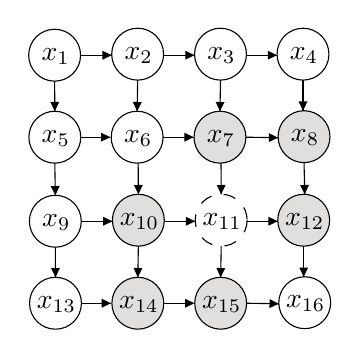
\begin{tikzpicture}[x=0.75pt,y=0.75pt,yscale=-0.5,xscale=0.5]
%uncomment if require: \path (0,426); %set diagram left start at 0, and has height of 426

\draw    (45.2, 36.5) circle [x radius= 25, y radius= 25]  ;
\draw    (125.2, 35.5) circle [x radius= 25, y radius= 25]  ;
\draw    (70.7,36.5) -- (100.2,36.5) ;
\draw [shift={(100.2,36.5)}, rotate = 180] [fill={rgb, 255:red, 0; green, 0; blue, 0 }  ] [draw opacity=0] (8.93,-4.29) -- (0,0) -- (8.93,4.29) -- (8.93,-4.29)    ;

\draw    (45.37, 115.5) circle [x radius= 25, y radius= 25]  ;
\draw    (124.7, 115.5) circle [x radius= 25, y radius= 25]  ;
\draw    (205.03, 35.5) circle [x radius= 25, y radius= 25]  ;
\draw    (284.53, 35.5) circle [x radius= 25, y radius= 25]  ;
\draw  [fill={rgb, 255:red, 225; green, 222; blue, 222 }  ,fill opacity=1 ]  (204.53, 115.5) circle [x radius= 25, y radius= 25]  ;
\draw  [fill={rgb, 255:red, 225; green, 222; blue, 222 }  ,fill opacity=1 ]  (285.53, 115) circle [x radius= 25, y radius= 25]  ;
\draw    (205.03,60.5) -- (204.53,90.5) ;
\draw [shift={(204.53,90.5)}, rotate = 270.95] [fill={rgb, 255:red, 0; green, 0; blue, 0 }  ] [draw opacity=0] (8.93,-4.29) -- (0,0) -- (8.93,4.29) -- (8.93,-4.29)    ;

\draw    (45.2,61.5) -- (45.37,90.5) ;
\draw [shift={(45.37,90.5)}, rotate = 269.67] [fill={rgb, 255:red, 0; green, 0; blue, 0 }  ] [draw opacity=0] (8.93,-4.29) -- (0,0) -- (8.93,4.29) -- (8.93,-4.29)    ;

\draw    (45.37,140.5) -- (45.87,171.5) ;
\draw [shift={(45.87,171.5)}, rotate = 269.08] [fill={rgb, 255:red, 0; green, 0; blue, 0 }  ] [draw opacity=0] (8.93,-4.29) -- (0,0) -- (8.93,4.29) -- (8.93,-4.29)    ;

\draw    (70.37,115.5) -- (98.87,115.5) ;
\draw [shift={(98.87,115.5)}, rotate = 180] [fill={rgb, 255:red, 0; green, 0; blue, 0 }  ] [draw opacity=0] (8.93,-4.29) -- (0,0) -- (8.93,4.29) -- (8.93,-4.29)    ;

\draw    (150.53,36.5) -- (180.03,36.5) ;
\draw [shift={(180.03,36.5)}, rotate = 180] [fill={rgb, 255:red, 0; green, 0; blue, 0 }  ] [draw opacity=0] (8.93,-4.29) -- (0,0) -- (8.93,4.29) -- (8.93,-4.29)    ;

\draw    (230.03,36.5) -- (259.53,36.5) ;
\draw [shift={(259.53,36.5)}, rotate = 180] [fill={rgb, 255:red, 0; green, 0; blue, 0 }  ] [draw opacity=0] (8.93,-4.29) -- (0,0) -- (8.93,4.29) -- (8.93,-4.29)    ;

\draw    (149.7,115.5) -- (179.2,115.5) ;
\draw [shift={(179.2,115.5)}, rotate = 180] [fill={rgb, 255:red, 0; green, 0; blue, 0 }  ] [draw opacity=0] (8.93,-4.29) -- (0,0) -- (8.93,4.29) -- (8.93,-4.29)    ;

\draw    (125.2,60.5) -- (124.7,90.5) ;
\draw [shift={(124.7,90.5)}, rotate = 270.95] [fill={rgb, 255:red, 0; green, 0; blue, 0 }  ] [draw opacity=0] (8.93,-4.29) -- (0,0) -- (8.93,4.29) -- (8.93,-4.29)    ;

\draw    (284.53,60.5) -- (284.53,90) ;
\draw [shift={(284.53,90)}, rotate = 270] [fill={rgb, 255:red, 0; green, 0; blue, 0 }  ] [draw opacity=0] (8.93,-4.29) -- (0,0) -- (8.93,4.29) -- (8.93,-4.29)    ;

\draw    (229.53,115.5) -- (260.53,116) ;
\draw [shift={(260.53,116)}, rotate = 180.92] [fill={rgb, 255:red, 0; green, 0; blue, 0 }  ] [draw opacity=0] (8.93,-4.29) -- (0,0) -- (8.93,4.29) -- (8.93,-4.29)    ;

\draw    (45.87, 196.5) circle [x radius= 25, y radius= 25]  ;
\draw  [fill={rgb, 255:red, 225; green, 222; blue, 222 }  ,fill opacity=1 ]  (125.87, 195.5) circle [x radius= 25, y radius= 25]  ;
\draw    (71.37,196.5) -- (100.87,196.5) ;
\draw [shift={(100.87,196.5)}, rotate = 180] [fill={rgb, 255:red, 0; green, 0; blue, 0 }  ] [draw opacity=0] (8.93,-4.29) -- (0,0) -- (8.93,4.29) -- (8.93,-4.29)    ;

\draw    (46.03, 275.5) circle [x radius= 25, y radius= 25]  ;
\draw  [fill={rgb, 255:red, 225; green, 222; blue, 222 }  ,fill opacity=1 ]  (125.37, 275.5) circle [x radius= 25, y radius= 25]  ;
\draw  [dash pattern={on 4.5pt off 4.5pt}]  (205.7, 195.5) circle [x radius= 25, y radius= 25]  ;
\draw  [fill={rgb, 255:red, 225; green, 222; blue, 222 }  ,fill opacity=1 ]  (285.2, 195.5) circle [x radius= 25, y radius= 25]  ;
\draw  [fill={rgb, 255:red, 225; green, 222; blue, 222 }  ,fill opacity=1 ]  (205.2, 275.5) circle [x radius= 25, y radius= 25]  ;
\draw    (286.2, 275) circle [x radius= 25, y radius= 25]  ;
\draw    (205.7,220.5) -- (205.2,250.5) ;
\draw [shift={(205.2,250.5)}, rotate = 270.95] [fill={rgb, 255:red, 0; green, 0; blue, 0 }  ] [draw opacity=0] (8.93,-4.29) -- (0,0) -- (8.93,4.29) -- (8.93,-4.29)    ;

\draw    (45.87,221.5) -- (46.03,250.5) ;
\draw [shift={(46.03,250.5)}, rotate = 269.67] [fill={rgb, 255:red, 0; green, 0; blue, 0 }  ] [draw opacity=0] (8.93,-4.29) -- (0,0) -- (8.93,4.29) -- (8.93,-4.29)    ;

\draw    (71.03,275.5) -- (99.53,275.5) ;
\draw [shift={(99.53,275.5)}, rotate = 180] [fill={rgb, 255:red, 0; green, 0; blue, 0 }  ] [draw opacity=0] (8.93,-4.29) -- (0,0) -- (8.93,4.29) -- (8.93,-4.29)    ;

\draw    (151.2,196.5) -- (180.7,196.5) ;
\draw [shift={(180.7,196.5)}, rotate = 180] [fill={rgb, 255:red, 0; green, 0; blue, 0 }  ] [draw opacity=0] (8.93,-4.29) -- (0,0) -- (8.93,4.29) -- (8.93,-4.29)    ;

\draw    (230.7,196.5) -- (260.2,196.5) ;
\draw [shift={(260.2,196.5)}, rotate = 180] [fill={rgb, 255:red, 0; green, 0; blue, 0 }  ] [draw opacity=0] (8.93,-4.29) -- (0,0) -- (8.93,4.29) -- (8.93,-4.29)    ;

\draw    (150.37,275.5) -- (179.87,275.5) ;
\draw [shift={(179.87,275.5)}, rotate = 180] [fill={rgb, 255:red, 0; green, 0; blue, 0 }  ] [draw opacity=0] (8.93,-4.29) -- (0,0) -- (8.93,4.29) -- (8.93,-4.29)    ;

\draw    (125.87,220.5) -- (125.37,250.5) ;
\draw [shift={(125.37,250.5)}, rotate = 270.95] [fill={rgb, 255:red, 0; green, 0; blue, 0 }  ] [draw opacity=0] (8.93,-4.29) -- (0,0) -- (8.93,4.29) -- (8.93,-4.29)    ;

\draw    (285.2,220.5) -- (285.2,250) ;
\draw [shift={(285.2,250)}, rotate = 270] [fill={rgb, 255:red, 0; green, 0; blue, 0 }  ] [draw opacity=0] (8.93,-4.29) -- (0,0) -- (8.93,4.29) -- (8.93,-4.29)    ;

\draw    (230.2,275.5) -- (261.2,276) ;
\draw [shift={(261.2,276)}, rotate = 180.92] [fill={rgb, 255:red, 0; green, 0; blue, 0 }  ] [draw opacity=0] (8.93,-4.29) -- (0,0) -- (8.93,4.29) -- (8.93,-4.29)    ;

\draw    (125.7,140.5) -- (125.87,170.5) ;
\draw [shift={(125.87,170.5)}, rotate = 269.68] [fill={rgb, 255:red, 0; green, 0; blue, 0 }  ] [draw opacity=0] (8.93,-4.29) -- (0,0) -- (8.93,4.29) -- (8.93,-4.29)    ;

\draw    (285.53,140) -- (286.2,170.5) ;
\draw [shift={(286.2,170.5)}, rotate = 268.75] [fill={rgb, 255:red, 0; green, 0; blue, 0 }  ] [draw opacity=0] (8.93,-4.29) -- (0,0) -- (8.93,4.29) -- (8.93,-4.29)    ;

\draw    (205.53,140.5) -- (205.7,170.5) ;
\draw [shift={(205.7,170.5)}, rotate = 269.68] [fill={rgb, 255:red, 0; green, 0; blue, 0 }  ] [draw opacity=0] (8.93,-4.29) -- (0,0) -- (8.93,4.29) -- (8.93,-4.29)    ;


\draw (46.2,37.44) node   {$x_{1}$};
\draw (126.2,36.44) node   {$x_{2}$};
\draw (46.37,116.44) node   {$x_{5}$};
\draw (125.7,116.44) node   {$x_{6}$};
\draw (206.03,36.44) node   {$x_{3}$};
\draw (285.53,36.44) node   {$x_{4}$};
\draw (205.53,116.44) node   {$x_{7}$};
\draw (286.53,115.94) node   {$x_{8}$};
\draw (46.87,197.44) node   {$x_{9}$};
\draw (126.87,196.44) node   {$x_{10}$};
\draw (47.03,276.44) node   {$x_{13}$};
\draw (126.37,276.44) node   {$x_{14}$};
\draw (206.7,196.44) node   {$x_{11}$};
\draw (286.2,196.44) node   {$x_{12}$};
\draw (206.2,276.44) node   {$x_{15}$};
\draw (287.2,275.94) node   {$x_{16}$};


\end{tikzpicture}
}
\quad
\subfloat[]{\label{fig:dgm_ugm_b}\documentclass[../capitulos/cap1.tex]{subfiles}



\tikzset{every picture/.style={line width=0.75pt}} %set default line width to 0.75pt

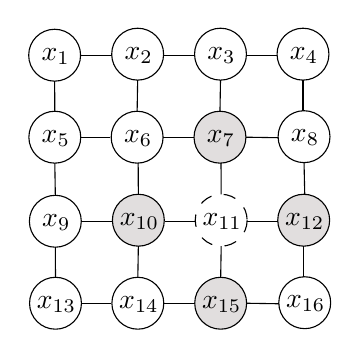
\begin{tikzpicture}[x=0.75pt,y=0.75pt,yscale=-0.5,xscale=0.5]
%uncomment if require: \path (0,426); %set diagram left start at 0, and has height of 426

\draw    (45.2, 36.5) circle [x radius= 25, y radius= 25]  ;
\draw    (125.2, 35.5) circle [x radius= 25, y radius= 25]  ;
\draw    (70.7,36.5) -- (100.2,36.5) ;


\draw    (45.37, 115.5) circle [x radius= 25, y radius= 25]  ;
\draw    (124.7, 115.5) circle [x radius= 25, y radius= 25]  ;
\draw    (205.03, 35.5) circle [x radius= 25, y radius= 25]  ;
\draw    (284.53, 35.5) circle [x radius= 25, y radius= 25]  ;
\draw  [fill={rgb, 255:red, 225; green, 222; blue, 222 }  ,fill opacity=1 ]  (204.53, 115.5) circle [x radius= 25, y radius= 25]  ;
\draw    (285.53, 115) circle [x radius= 25, y radius= 25]  ;
\draw    (205.03,60.5) -- (204.53,90.5) ;


\draw    (45.2,61.5) -- (45.37,90.5) ;


\draw    (45.37,140.5) -- (45.87,171.5) ;


\draw    (70.37,115.5) -- (98.87,115.5) ;


\draw    (150.53,36.5) -- (180.03,36.5) ;


\draw    (230.03,36.5) -- (259.53,36.5) ;


\draw    (149.7,115.5) -- (179.2,115.5) ;


\draw    (125.2,60.5) -- (124.7,90.5) ;


\draw    (284.53,60.5) -- (284.53,90) ;


\draw    (229.53,115.5) -- (260.53,116) ;


\draw    (45.87, 196.5) circle [x radius= 25, y radius= 25]  ;
\draw  [fill={rgb, 255:red, 225; green, 222; blue, 222 }  ,fill opacity=1 ]  (125.87, 195.5) circle [x radius= 25, y radius= 25]  ;
\draw    (71.37,196.5) -- (100.87,196.5) ;


\draw    (46.03, 275.5) circle [x radius= 25, y radius= 25]  ;
\draw    (125.37, 275.5) circle [x radius= 25, y radius= 25]  ;
\draw  [dash pattern={on 4.5pt off 4.5pt}]  (205.7, 195.5) circle [x radius= 25, y radius= 25]  ;
\draw  [fill={rgb, 255:red, 225; green, 222; blue, 222 }  ,fill opacity=1 ]  (285.2, 195.5) circle [x radius= 25, y radius= 25]  ;
\draw  [fill={rgb, 255:red, 225; green, 222; blue, 222 }  ,fill opacity=1 ]  (205.2, 275.5) circle [x radius= 25, y radius= 25]  ;
\draw    (286.2, 275) circle [x radius= 25, y radius= 25]  ;
\draw    (205.7,220.5) -- (205.2,250.5) ;


\draw    (45.87,221.5) -- (46.03,250.5) ;


\draw    (71.03,275.5) -- (99.53,275.5) ;


\draw    (151.2,196.5) -- (180.7,196.5) ;


\draw    (230.7,196.5) -- (260.2,196.5) ;


\draw    (150.37,275.5) -- (179.87,275.5) ;


\draw    (125.87,220.5) -- (125.37,250.5) ;


\draw    (285.2,220.5) -- (285.2,250) ;


\draw    (230.2,275.5) -- (261.2,276) ;


\draw    (125.7,140.5) -- (125.87,170.5) ;


\draw    (285.53,140) -- (286.2,170.5) ;


\draw    (205.53,140.5) -- (205.7,170.5) ;



\draw (46.2,37.44) node   {$x_{1}$};
\draw (126.2,36.44) node   {$x_{2}$};
\draw (46.37,116.44) node   {$x_{5}$};
\draw (125.7,116.44) node   {$x_{6}$};
\draw (206.03,36.44) node   {$x_{3}$};
\draw (285.53,36.44) node   {$x_{4}$};
\draw (205.53,116.44) node   {$x_{7}$};
\draw (286.53,115.94) node   {$x_{8}$};
\draw (46.87,197.44) node   {$x_{9}$};
\draw (126.87,196.44) node   {$x_{10}$};
\draw (47.03,276.44) node   {$x_{13}$};
\draw (126.37,276.44) node   {$x_{14}$};
\draw (206.7,196.44) node   {$x_{11}$};
\draw (286.2,196.44) node   {$x_{12}$};
\draw (206.2,276.44) node   {$x_{15}$};
\draw (287.2,275.94) node   {$x_{16}$};


\end{tikzpicture}
}
\quad
\caption{ Modelo gráfico dirigido (izquierda) contrapuesto a uno no dirigido (derecha). En \subref{fig:dgm_ugm_a} el markov blanket de $x_{11}$ añade a $x_8$ y $x_{14}$ a sus vecinos inmediatos, mientras excluye a $x_6$ y $x_16$ en aplicaciones basadas en imágenes, este comportamiento puede no ser el deseado. Por otra parte en \subref{fig:dgm_ugm_b} el nodo $x_{11}$ esta separado del resto solo por sus vecinos inmediatos.}
\end{figure}



\section{Inferencia exacta en modelos gráficos}
